\documentclass[oneside,11pt,a4paper]{article}

% Chargement d'extensions
\usepackage[utf8]{inputenc}
\usepackage[french]{babel}
\usepackage[T1]{fontenc}
\usepackage{graphicx}
\usepackage[top=3cm, bottom=3cm, left=3cm, right=3cm]{geometry}
% Bout de code
\usepackage{listings}
\usepackage{color}

\definecolor{mygreen}{rgb}{0,0.6,0}
\definecolor{mygray}{rgb}{0.5,0.5,0.5}
\definecolor{mymauve}{rgb}{0.58,0,0.82}

% Commande pour notation 'NB :' (nota bene)
\newcommand\nb[1][0.3]{N\kern-#1emB : }

% csquotes va utiliser la langue définie dans babel
\usepackage[babel=true]{csquotes}

% pour afficher Schéma au lieu de figure dans les legende des images
\addto\captionsfrench{\def\figurename{Schéma}}

% stylisation des enumerations
\frenchbsetup{StandardLists=false} 
\usepackage{enumitem}

% utilisation de lorem lipsum
\usepackage{lipsum}

% Informations le titre, le(s) auteur(s), la date
\title{Hérault Events}
\author{
    Chakib ELHOUITI \and
    Massili KEZZOUL 
}
\date{\today}


\begin{document}
%\maketitle
\begin{titlepage}
	\centering
	{\scshape\LARGE Universite de Montpellier\par}
	{\scshape\Large Rapport de projet Base de données HLIN511\par}
	\vspace{1.5cm}
	{\huge\bfseries Hérault Events\par}
	\vspace{2cm}
	
	{\Large\itshape
		Chakib ELHOUITI : 21813619\\
		Massili KEZZOUL : 21815514\\
		Groupe P \\
		\par}

	\vspace{2cm}
	
	\begin{figure}[h]
		\begin{minipage}[c]{.30\linewidth}
			\centering
			
\includegraphics[width=1\textwidth]{img/um.png}
		\end{minipage}
		\hfill
		\begin{minipage}[c]{.30\linewidth}
			\centering
			
\includegraphics[width=1\textwidth]{img/HE-noir.png}
		\end{minipage}
		\hfill
		\begin{minipage}[c]{.30\linewidth}
			\centering
			
\includegraphics[width=1\textwidth]{img/fds.png}
		\end{minipage}
	\end{figure}

	\vspace{1.5cm}

\vfill
	% Bottom of the page
	{\large \today\par}
\end{titlepage}
\section{Introduction}

Dans le cadre d'un projet commun entre deux UE de la faculté des sciences de l'univérsite de Montpellier, nous avons réaliser une base de données associée à une application web permettant la publication d’événements culturels ou sportifs dans un département donné. Nous avons choisi le département de l'Hérault. L'application peut d'ailleur être visitée à cette adresse `http://webpeda.etu.umontpellier.fr/e20180011096` à condition d'être sur le réseau de l'univérsite de Montepellier.

\section{Modèl entité-association}

\subsection{Schéma E/A}

Tout d'abord nous avons modélisé notre base de données de la manière suivante :

\begin{figure}[h]
  \centering
  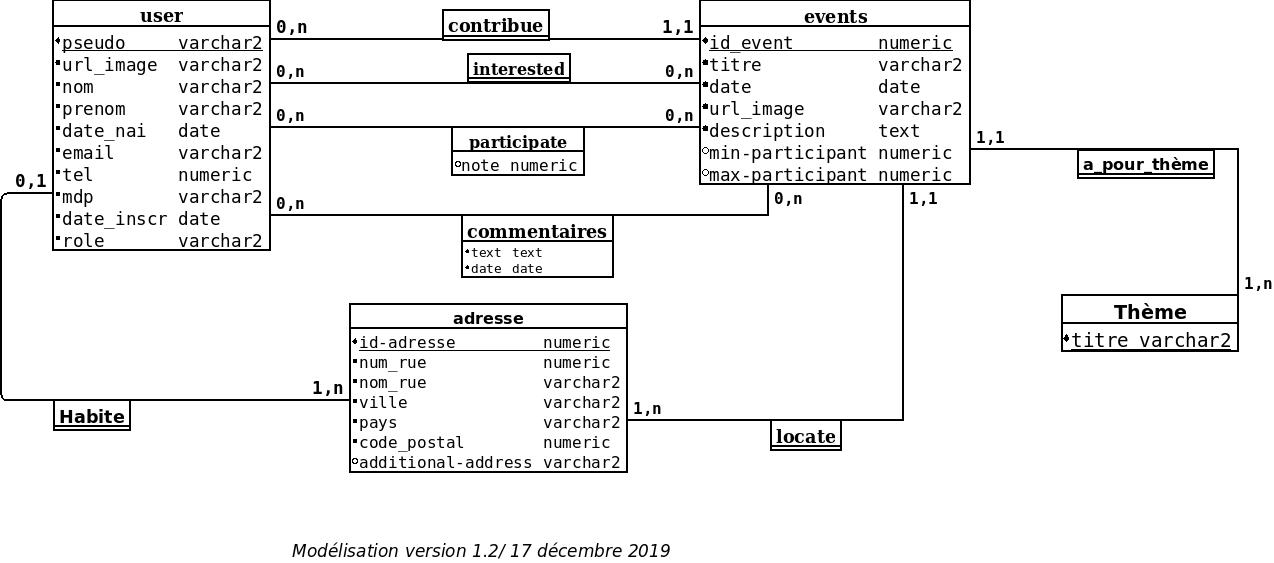
\includegraphics[width=1\textwidth]{img/modelisation.jpeg}
  \caption{Modèl E/A}
\end{figure}

\subsection{Explication du Scéma}

\subsubsection*{Les tables}

\begin{description}
	\item[Adresse :] Cette table permet de stocker l'ensemble des adresses qui seront utilisés par la table \textit{User} et \textit{Events}. On a choisi de ne pas stocker les coordonnées GPS des adresses car ils peuvent être calculés (par une API par example). On a decidé de le faire de cette manière aussi parcequ'il est préferable de ne pas demander des coordonnées GPS à un utilisateur lambda de l'application web.
	\item[User :] La table \textit{User} stock les informations personnelles des utilisateurs du site web. Un utilisateur est identifié par un pseudo qu'il renseigne à son inscription. Ce dernier doit bien évidement être unique.\\ Il existe trois types d'utilisateur : 
	\begin{itemize}[label=\textbullet, font=\small \color{mygray}]
		\item Visiteur ('visitor')
		\item Contributeur ('contributor')
		\item Administrateur ('admin')
	\end{itemize}
	Le type de chaque utilisateur est stocké dans l'attribut \textit{role\_user} qui est une énumération ( de type ENUM ).
	L'attribut \textit{email}, et \textit{tel} doivent être unique.
	\item[Events :] Cette table se charge de stocker les informations relatifs à un événement. Un événement est défini par un identificateur numéric qui générer automatiquement à l'insertion d'un tuple (par AUTO\_INCREMENT) et contient forcément un titre et une date (attribut de type DATETIME). Il peut aussi contenir un lien vers une image (local ou distante), une description (de type TEXT) et un nombre minimum et maximum de participant.
	\item[Theme :] Chaque événement est organisé autour d'un théme donné, donc on a aussi modélisé une table thème afin de stocker tout les thèmes. 
\end{description}

\subsubsection*{Les association}

\begin{description}
	\item[Contribue : ] zeb zeb zeb \lipsum[1]
	\item[Participate : ] zeb zeb zeb \lipsum[1]
	\item[Interested : ] zeb zeb zeb \lipsum[1]
	\item[Commentaire : ] zeb zeb zeb \lipsum[1]
	\item[Habite : ] zeb zeb zeb \lipsum[1]
	\item[Locate : ] zeb zeb zeb \lipsum[1]
	\item[A\_pour\_themes : ] zeb zeb zeb \lipsum[1]
\end{description}

\subsection{Modèle logique de données}

\lipsum[1]

\section{Les procédures}

Puis pour mieux structurer les differents fichiers sources nous avons decidé d'utiliser la structure MVC (pour Model View Controller). Nous avons donc stocker tout nos fichiers dans trois dossiers : Model, View et Controller. Les fichiers du model se charge d'intéragir avec la base de données, les fichiers dans le dossier view se charge d'afficher et de donnez du style à nos pages, enfin les fichiers du dossier Controller fait la liason entre le model et les View. (voir : https://fr.wikipedia.org/wiki/Mod\%C3\%A8le-vue-contr\%C3\%B4leur).


Vu le temps qu'il nous a été accordé, on a décidé d'écrire tout les codes sources de zéro (from Scratch) sans utiliser de framework. 
Les fichiers css on été écrit en SASS.

\section{Les triggers}

Sur toutes les foncionnalitées demandées, nous les avons toutes implementées sauf :

\begin{itemize}
  \item La visualisation de tout les événements en mode cartographique, néanmoins nous avons pu implementées dans la page d'un seul événement donné, sa position dans une carte (avec OpenLayers).
\end{itemize}

Par contre, nous avons implementé la possibilité pour un utilisateur, une fois inscrit, de modifier ses informations personnels, ajouter une photo pour son profil et aussi la possibilité de supprimer son compte.

On a aussi ajouté la possibilité pour un utilisateur de s'interessé à un événement avant d'y participer.

\section{Les fonctions}

\section{Conclusion}

\subsection{Les problèmes recontrés}

Lors du développement du projet, nous n'avons rencontré aucun problème particulier. En revanche lors du déploiment de l'application sur le serveur de la faculté des sciences, nous avons recontrés deux problèmes que nous n'avons pas pu résoudre.

\begin{itemize}
	\item La fonction PHP `curl\_exec()` qui permet de récuperer des données via des requêtes HTTP ne fonctionne pas. ce qui est génant car elle nous permet de récuperer les coordonnées GPS d'une adresse donnée. (la map ne fonctionne donc pas sur le serveur de la fac)
	\item Le serveur ne nous permet pas d'uploader des images. Il est donc impossible de mettre des images de profil et des images pour des événements.
\end{itemize}

\subsection{Les compètences acquises}

Pour conclure, à l’issue de ce projet nous avons réussi à réaliser un site web fonctionnel et prèt à l'utilisation. 

Ce projet nous aura permis d’aprofondir nos connaissances en développement web et de compléter nos acquis sur les outils de base du web, tel que :HTML, CSS, PHP et JAVASCRIPT.

\end{document}
